\documentclass[conference]{IEEEtran}
\IEEEoverridecommandlockouts
\usepackage{cite}
\usepackage{amsmath,amssymb,amsfonts}
\usepackage{algorithmic}
\usepackage{graphicx}
\usepackage{textcomp}
\usepackage{xcolor}
\usepackage{booktabs}
\usepackage{array}
\usepackage{url}
\usepackage{tikz}
\usetikzlibrary{shapes.geometric, arrows.meta, positioning, calc, backgrounds}
\usepackage{fancyhdr}
\usepackage{hyperref}
\hypersetup{hidelinks}

\fancypagestyle{firstpage}{
  \fancyhf{}
  \fancyhead[C]{23rd Edition of IEEE India Council International Conference (INDICON 2026)}
  \fancyfoot[L]{%
      \begin{minipage}[t]{\textwidth}
      \normalsize{979-8-3195-2581-9/26/\$31.00 \copyright2026 IEEE}
    \end{minipage}%
  }
  \renewcommand{\headrulewidth}{0pt}
}

\pagestyle{fancy}
\fancyhf{}
\fancyfoot[C]{INDICON 2026}
\renewcommand{\headrulewidth}{0pt}


\begin{document}
\title{Route-Aware Dead Reckoning and Road-Scene Segmentation for Smart-Helmet Two-Wheeler Navigation Under GNSS Denial}

\author{\IEEEauthorblockN{Jinesh Nanal\textsuperscript{*}}
\IEEEauthorblockA{\textit{School of Computer Engineering and Technology} \\
\textit{MIT World Peace University}\\
Pune, India \\
jineshnanal04@gmail.com}
\and
\IEEEauthorblockN{Priyal Jain}
\IEEEauthorblockA{\textit{School of Computer Engineering and Technology} \\
\textit{MIT World Peace University}\\
Pune, India \\
priyal2004jain@gmail.com}
}

\maketitle
\thispagestyle{firstpage}

\begin{abstract}
GNSS-based navigation becomes unreliable in tunnels, under flyovers and in dense urban areas, precisely where a missed turn is most costly. This paper proposes an offline navigation system that combines dead reckoning (DR) with camera-based road feature detection to help maintain the route when the GNSS signal becomes weak or unavailable. The system maintains a \emph{route pointer} over cached OpenStreetMap data and advances it from two complementary signals: distance-based progression from DR, and semantic road-feature events from a forward-facing camera that act as correction anchors resetting accumulated drift; when vision is unreliable, DR carries the pointer until the next reliable event. The framework is realised as a smart-helmet prototype that streams camera and inertial sensing over a compact 8-byte Bluetooth Low Energy link to a companion phone running route logic on cached assets. We validate on recorded road data rather than in simulation: a four-configuration ablation over 47 paired GNSS blackouts drawn from an instrumented 2.76\,km two-wheeler ride shows that the complete system reduces peak position error by 19.7\,\% against unaided dead reckoning ($p{=}0.002$), while junction correction without route context confers no measurable benefit ($p{=}0.26$). The result holds in 23 of 24 threshold settings and is reproduced on six further rides, including a flyover and an underpass (20.6\,\% over all 85 windows, $p{<}0.001$). The segmentation model was trained using Indian road images and achieved a road intersection-over-union (IoU) of 0.856 on unseen BDD100K data. It was able to detect the road ahead in 54 out of 56 helmet-camera frames and took 15.7\,ms to run on the connected smartphone.
\end{abstract}

\begin{IEEEkeywords}
Offline navigation, dead reckoning, GNSS-denied localisation, map matching, road segmentation, smart helmet, two-wheeler safety.
\end{IEEEkeywords}

% ==============================================================
\section{Introduction}
% ==============================================================

Road navigation is now overwhelmingly dependent on Global Navigation Satellite System (GNSS) fixes together with network-assisted map services. In tunnels, under flyovers and in dense urban canyons, both assumptions fail: the location estimate drifts, turn instructions are delayed or wrong, and the rider misses decision points. The problem is acute for two-wheeler riders, who cannot safely keep glancing at a phone screen.

This paper argues that \emph{continuity}, rather than raw coordinate accuracy, is the operationally correct primary objective for rider-facing navigation on two-wheelers. We describe a prototype smart-helmet stack combining dead reckoning (DR) for short-term motion propagation with a lightweight computer-vision (CV) module that detects navigation-relevant road features (turns, T-junctions, cross intersections, forks, roundabout entries) as \emph{semantic correction events} for a route pointer maintained over cached OpenStreetMap (OSM) data.

\emph{Contributions.} \textbf{C1:} The system uses road features detected by the camera as correction points for the route pointer maintained through dead reckoning, instead of relying on continuous localisation. It also supports online, offline and degraded modes to keep the navigation interface stable when the GNSS signal is weak or unavailable. \textbf{C2:} The helmet sends camera and inertial measurement unit (IMU) data to the phone using 8-byte Bluetooth Low Energy (BLE) packets. Checksums and acknowledgements (ACKs) are used to check whether the data is received correctly, while keeping the helmet's power consumption low. \textbf{C3:} The system was tested using real road data, including a four-configuration ablation study with paired GNSS blackouts from seven recorded rides. The evaluation also includes road segmentation tests on BDD100K, 56 helmet-camera frames, performance measurements on the phone and 138 unit tests.

% ==============================================================
\section{Related Work}
\label{sec:related}
% ==============================================================

In~\cite{javed2025arc}, arc-length map matching helps keep the vehicle on the road graph and reduces drift from dead reckoning when GNSS is unavailable. In~\cite{wang2025gnss}, GNSS, IMU and map matching are used together to adjust how much the system trusts noisy GNSS signals in urban canyons. Both approaches use road and route geometry to understand movement, which is also the idea behind our route pointer. Visual localisation matches onboard imagery to satellite maps~\cite{lin2025gnss}, learns place-recognition descriptors~\cite{li2024cspformer,he2026guiding}, or uses temporally consistent visual cues as corrections~\cite{xu2026enhanced,shpagin2026naviloc,wang2026particle}, but most methods need reference databases or computation that is heavy for continuous mobile use. Classical cues such as HOG~\cite{dalal2005hog} and Canny edges~\cite{canny1986} remain cheap, while the LR-ASPP decoder on MobileNetV3~\cite{howard2019searching} and the India Driving Dataset~\cite{iddvarma2019} make mobile road segmentation practical on Indian roads. These works optimise coordinate estimates and assume continuous sensing; less attention is paid to what keeps guidance usable on a moving two-wheeler, namely explicit online/offline transitions, degraded-mode behaviour and stable rider cues. This paper addresses that gap, with guidance driven by semantic events, such as a turn observed or a junction recognised, rather than by metric fixes.

% ==============================================================
\section{System Architecture}
\label{sec:arch}
% ==============================================================

Following the layered-plant view that ISA-95 uses for industrial automation, we organise the smart-helmet software into four cooperating layers that separate what is being sensed from how a decision is presented to the rider (Fig.~\ref{fig:arch}).

\begin{figure*}[t]
\centering
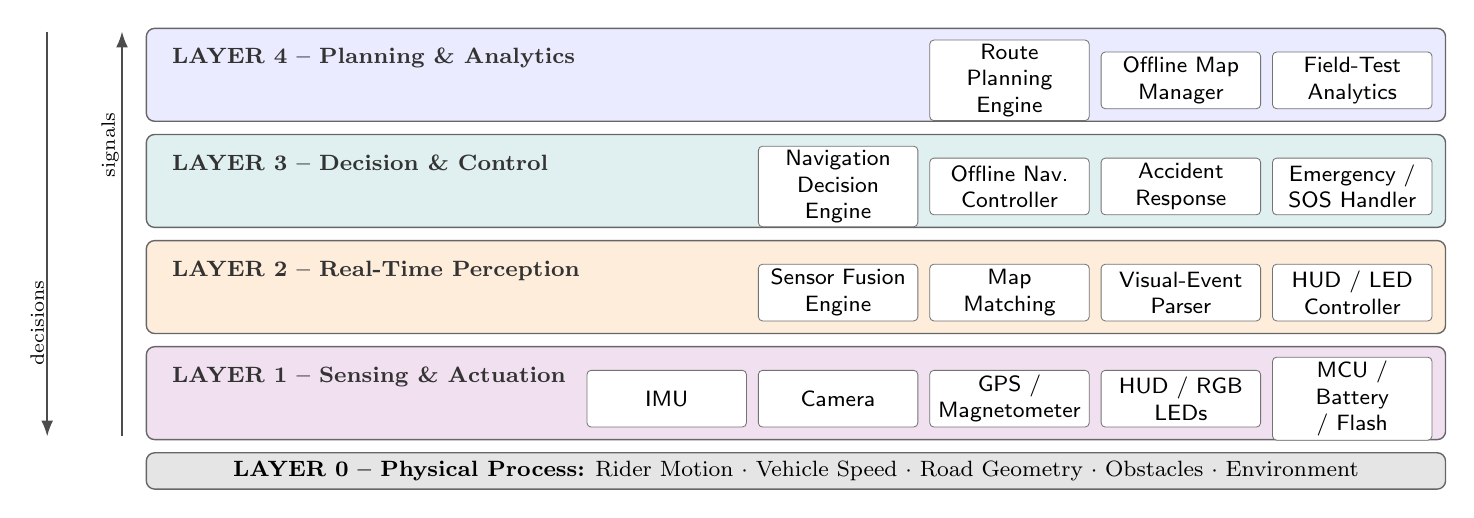
\begin{tikzpicture}[
    font=\footnotesize\sffamily,
    layertitle/.style={font=\footnotesize\bfseries, text=black!80},
    mod/.style={rectangle, rounded corners=1.5pt, draw=black!55, fill=white,
                line width=0.3pt, minimum height=0.72cm, text width=1.92cm,
                align=center, inner sep=1.5pt},
    band/.style={rectangle, rounded corners=3pt, draw=black!60, line width=0.5pt,
                 minimum width=16.5cm, minimum height=1.18cm, inner sep=3pt},
    procbar/.style={rectangle, rounded corners=3pt, draw=black!60, fill=black!10,
                    line width=0.5pt, minimum width=16.5cm, minimum height=0.46cm,
                    inner sep=3pt, font=\footnotesize},
    arr/.style={-{Latex[length=2mm]}, semithick, black!70}
]
% ---- Layer bands ----
\node[band, fill=blue!8]                       (b4) {};
\node[band, fill=teal!12,   below=0.15cm of b4] (b3) {};
\node[band, fill=orange!14, below=0.15cm of b3] (b2) {};
\node[band, fill=violet!12, below=0.15cm of b2] (b1) {};
\node[procbar,              below=0.15cm of b1] (b0)
     {\textbf{LAYER 0 -- Physical Process:} Rider Motion $\cdot$ Vehicle Speed $\cdot$
      Road Geometry $\cdot$ Obstacles $\cdot$ Environment};

% ---- Layer titles ----
\node[layertitle, anchor=north west, xshift=6pt, yshift=-4pt]
      at (b4.north west) {LAYER 4 -- Planning \& Analytics};
\node[layertitle, anchor=north west, xshift=6pt, yshift=-4pt]
      at (b3.north west) {LAYER 3 -- Decision \& Control};
\node[layertitle, anchor=north west, xshift=6pt, yshift=-4pt]
      at (b2.north west) {LAYER 2 -- Real-Time Perception};
\node[layertitle, anchor=north west, xshift=6pt, yshift=-4pt]
      at (b1.north west) {LAYER 1 -- Sensing \& Actuation};

% ---- Modules per layer, right-anchored inside each band ----
% Layer 4 (3)
\node[mod, anchor=east, xshift=-5pt, yshift=-2pt] at (b4.east) (m43) {Field-Test\\Analytics};
\node[mod, left=4pt of m43] (m42) {Offline Map\\Manager};
\node[mod, left=4pt of m42] (m41) {Route Planning\\Engine};
% Layer 3 (4)
\node[mod, anchor=east, xshift=-5pt, yshift=-2pt] at (b3.east) (m34) {Emergency /\\SOS Handler};
\node[mod, left=4pt of m34] (m33) {Accident\\Response};
\node[mod, left=4pt of m33] (m32) {Offline Nav.\\Controller};
\node[mod, left=4pt of m32] (m31) {Navigation\\Decision Engine};
% Layer 2 (4)
\node[mod, anchor=east, xshift=-5pt, yshift=-2pt] at (b2.east) (m24) {HUD / LED\\Controller};
\node[mod, left=4pt of m24] (m23) {Visual-Event\\Parser};
\node[mod, left=4pt of m23] (m22) {Map\\Matching};
\node[mod, left=4pt of m22] (m21) {Sensor Fusion\\Engine};
% Layer 1 (5)
\node[mod, anchor=east, xshift=-5pt, yshift=-2pt] at (b1.east) (m15) {MCU / Battery\\/ Flash};
\node[mod, left=4pt of m15] (m14) {HUD / RGB\\LEDs};
\node[mod, left=4pt of m14] (m13) {GPS /\\Magnetometer};
\node[mod, left=4pt of m13] (m12) {Camera};
\node[mod, left=4pt of m12] (m11) {IMU};

% ---- Vertical flow arrows on the far left of the stack ----
\coordinate (upA) at ($(b1.south west)+(-0.30cm, 0.05cm)$);
\coordinate (upB) at ($(b4.north west)+(-0.30cm,-0.05cm)$);
\draw[arr] (upA) -- (upB);
\node[rotate=90, font=\scriptsize, anchor=south, inner sep=1pt]
      at ($(upA)!0.72!(upB)$) {signals};
\coordinate (dnA) at ($(b4.north west)+(-1.25cm,-0.05cm)$);
\coordinate (dnB) at ($(b1.south west)+(-1.25cm, 0.05cm)$);
\draw[arr] (dnA) -- (dnB);
\node[rotate=90, font=\scriptsize, anchor=south, inner sep=1pt]
      at ($(dnA)!0.72!(dnB)$) {decisions};
\end{tikzpicture}
\caption{The smart helmet uses a four-layer architecture inspired by ISA-95. Layer~0 represents the physical process, Layer~1 handles sensing and actuation, Layer~2 processes and interprets the data, Layer~3 makes decisions, and Layer~4 manages planning and logging. Signals move upward through the layers, turning raw data into meaningful events, while decisions move downward as simple cues for the rider.}
\label{fig:arch}
\end{figure*}

% ==============================================================
\section{Methods}
\label{sec:methods}
% ==============================================================

\subsection{Route pointer over cached OSM data}
The route is a cached sequence of expected map features, e.g.\ \textsc{start} $\rightarrow$ \textsc{straight} $\rightarrow$ \textsc{left-turn} $\rightarrow$ \textsc{t-junction} $\rightarrow$ \textsc{right-turn} $\rightarrow$ \textsc{destination}. The navigation module maintains a \emph{route pointer} over this sequence: DR advances it by estimated arc-length distance, the CV module reports confirmed features, and on a confidence-thresholded match with the next expected feature the pointer is updated and the DR uncertainty term is reset.

\subsection{Orientation and heading estimation}
Let $\mathbf{a}=(a_x,a_y,a_z)$ denote the accelerometer reading and $\boldsymbol{\omega}=(\omega_x,\omega_y,\omega_z)$ the gyroscope reading at time $t$. A complementary filter combines the drift-free but noisy tilt estimate from the accelerometer with the smooth but drifting angular integral from the gyroscope:
\begin{equation}
\theta(t) = \alpha\,\big(\theta(t{-}1) + \omega\,\Delta t\big) + (1-\alpha)\,\operatorname{atan2}(a_y, a_z),
\label{eq:cf}
\end{equation}
where, in \eqref{eq:cf}, $\alpha \in [0.9, 0.98]$ is tuned empirically for rider-mounted inertial measurement units (IMUs). A moving-window smoother is applied to $\theta$ to reject brief spikes exceeding a configured threshold.

\subsection{Dead reckoning}
Given filtered heading $\theta(t)$, estimated forward speed $v(t)$, and elapsed interval $\Delta t$, position is propagated as
\begin{align}
v(t) &= v(t{-}1) + \big(a_x - g\sin\theta\big)\,\Delta t,
\label{eq:dr_speed}\\
x(t) &= x(t{-}1) + v(t)\,\Delta t\,\cos\theta,\\
y(t) &= y(t{-}1) + v(t)\,\Delta t\,\sin\theta.
\label{eq:dr_pos}
\end{align}
Equations \eqref{eq:dr_speed}--\eqref{eq:dr_pos} propagate the estimate between position fixes. An uncertainty term $\sigma(t)$ grows linearly with cumulative travel under DR and is reset when the Global Positioning System (GPS) fix recovers or a visual event of sufficient confidence is accepted.

\subsection{Route-aware map matching}
Rather than snapping $(x,y)$ to the geometrically nearest road segment, we express position as arc-length progress $s$ along the currently active route polyline $\mathcal{R}$. For query point $\mathbf{p}=(x,y)$, $s = \arg\min_{s' \in [s_\text{curr}-\delta,\, s_\text{curr}+\delta]} \|\mathbf{p} - \mathcal{R}(s')\|_2$, where $\delta$ is a bounded window derived from the current DR uncertainty. This rules out physically implausible jumps to parallel roads, which a naive nearest-neighbour matcher cannot prevent in dense urban layouts.

\subsection{Computer-vision module}
The CV module only identifies which navigation-related feature is present in the current scene. It does not calculate object distances, control the vehicle, or localise it by itself. Instead, it gives its output as an event in the format \{\texttt{feature\_type}, \texttt{subtype}, \texttt{confidence}\}, while the navigation layer handles localisation.

\emph{(a) Road-topology pipeline.} Each frame goes through the following steps: frame $\rightarrow$ road segmentation $\rightarrow$ bird's-eye view (BEV) transformation $\rightarrow$ skeleton extraction $\rightarrow$ graph construction $\rightarrow$ junction-type classification. An LR-ASPP--MobileNetV3-Large network~\cite{howard2019searching}, trained on IDD classes~\cite{iddvarma2019}, generates a mask of the drivable road. This mask is transformed into a BEV view, making turns, branches and junctions easier to identify. Skeletonisation then reduces the mask to a one-pixel-wide centreline. A graph is built from this line, with road branches as edges and junction points as nodes. A node with degree three indicates a T-junction or fork, while degree four indicates a cross intersection. Alongside this, TinySceneCNN classifies the scene into eight classes (straight, left turn, right turn, junction, T-intersection, roundabout entry, occluded and other), providing an additional scene label with a confidence score.

\emph{(b) Temporal fusion.} All CV outputs are checked using a sliding-window vote across a few frames. A junction type is confirmed only if it stays above the threshold set for that class throughout the window. A short occlusion buffer allows a few missed frames without breaking continuity, while filtering out temporary false detections before they affect navigation.

\subsection{Navigation decision, mode transitions and confidence}
The decision engine uses a confidence tracker with three modes: \textsc{online}, \textsc{offline} and \textsc{degraded} (Fig.~\ref{fig:fsm}). It considers three inputs: GPS accuracy reported by the phone, dead-reckoning uncertainty ($\sigma$), and visual events that match the expected next turn. When a turn event passes the required threshold and the expected manoeuvre is within 15\,m along the route, the engine moves to the next manoeuvre, resets $\sigma$ and sends a cue to the helmet. Mode changes are also shown in the mobile app, so the rider knows which source of information is being trusted. This also prevents outdated navigation instructions from being displayed without a warning.

\begin{figure}[t]
\centering
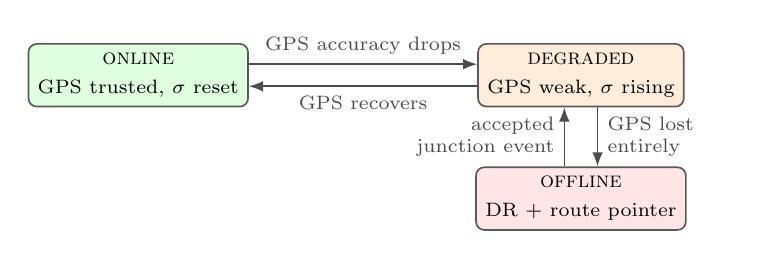
\begin{tikzpicture}[
    font=\footnotesize,
    state/.style={rectangle, rounded corners=3pt, draw=black!65, line width=0.6pt,
                  minimum width=1.85cm, minimum height=0.72cm, align=center},
    trans/.style={-{Latex[length=1.8mm]}, semithick, black!70},
    lbl/.style={font=\scriptsize, align=center, text width=2.5cm}
]
\node[state, fill=green!12]  (on)  {\textsc{online}\\[1pt]\scriptsize GPS trusted, $\sigma$ reset};
\node[state, fill=orange!14, right=2.9cm of on]  (deg) {\textsc{degraded}\\[1pt]\scriptsize GPS weak, $\sigma$ rising};
\node[state, fill=red!10, below=0.75cm of deg] (off) {\textsc{offline}\\[1pt]\scriptsize DR + route pointer};

\draw[trans] ([yshift=4pt]on.east) -- node[lbl, above] {GPS accuracy drops} ([yshift=4pt]deg.west);
\draw[trans] ([yshift=-4pt]deg.west) -- node[lbl, below] {GPS recovers} ([yshift=-4pt]on.west -| on.east);
\draw[trans] ([xshift=6pt]deg.south) -- node[lbl, right, text width=1.5cm, align=left] {GPS lost\\entirely} ([xshift=6pt]off.north);
\draw[trans] ([xshift=-6pt]off.north) -- node[lbl, left, text width=1.9cm, align=right] {accepted\\junction event} ([xshift=-6pt]deg.south);
\end{tikzpicture}
\caption{Confidence-tracker mode transitions. Junction events reset DR uncertainty $\sigma$ and can bring the system's confidence back towards the \textsc{online} level even without a GPS fix. The rider can always see the current mode and know which source of information is being used.}
\label{fig:fsm}
\end{figure}

\subsection{Helmet communication and SOS}
Important rider data is sent using fixed 8-byte BLE packets. Each packet contains a magic byte (\texttt{0xAB}), a type code for instruction, GPS status, speed, crash or heartbeat, a 2-byte sequence number, a 3-byte payload and an XOR checksum. The sequence number helps maintain packet order, remove duplicates and match ACKs. Heartbeat packets help detect when the connection is lost, and the packet parsing process takes constant time.

A pitch/roll threshold detector grades abnormal motion as \textsc{low}, \textsc{medium} or \textsc{critical}; on \textsc{critical}, the app calls and texts an emergency contact with the last-known location, and the helmet head-up display (HUD) shows a hazard cue.

% ==============================================================
\section{Experiments and Results}
\label{sec:eval}
% ==============================================================

\subsection{Prototype implementation}
The prototype consists of three main parts: (i) a forward-facing camera mounted on the helmet and a 6-axis IMU; (ii) an ESP32-based controller running a C/C++ sketch that packs sensor data into fixed 8-byte BLE frames and controls the light-emitting diode (LED) matrix and HUD using six command states for approach, execution, hazard and arrival cues; and (iii) a React~Native mobile app connected to a Python FastAPI backend that handles navigation, DR and CV. Routes are obtained from OSRM/Google Routes as encoded polylines and stored on the phone with per-turn information and OSM map tiles, allowing map matching and rider directions to continue offline. The segmentation model is trained on IDD~\cite{iddvarma2019}.

\subsection{Test coverage and results}
The unit-test suite includes 138 tests across three modules, with 133 passing (Table~\ref{tab:unit}). All five failures are in the navigation API-service suite and relate to unresolved degraded-mode transitions. These failures are reported rather than hidden. Another 10 scenario tests covering packet corruption, invalid IMU samples, heading spikes, off-route map matching, connection loss and end-to-end navigation also pass.

\begin{table}[t]
\centering
\caption{Module-wise unit-test outcome on the current prototype.}
\label{tab:unit}
\setlength{\tabcolsep}{3pt}
\begin{tabular}{@{}lcc@{}}
\toprule
\textbf{Module} & \textbf{Passed} & \textbf{Total}\\
\midrule
Communication & 24 & 24\\
Localisation  & 25 & 25\\
Navigation    & 84 & 89\\
\midrule
\textbf{Total} & \textbf{133} & \textbf{138}\\
\bottomrule
\end{tabular}
\end{table}


\subsection{Integrated pipeline behaviour}
Fig.~\ref{fig:pipeline_trace} shows a typical 60\,s GNSS blackout from the original ride. Dead reckoning alone drifts up to 254\,m due to heading errors and the assumption that speed remains constant. In comparison, the full system keeps the error within 72\,m. Junction events at 11\,s and 15\,s bring the pointer back onto the cached route, and map matching then keeps it within the route corridor. The ablation study measures this effect across all windows.

\begin{figure}[!t]
\centering
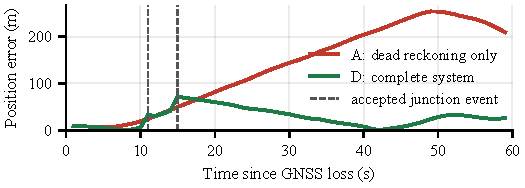
\includegraphics[width=\linewidth,keepaspectratio]{real_ride_trace.pdf}
\caption{Position error measured against GNSS ground truth during a typical 60\,s blackout from the recorded ride. Dead reckoning alone (A) drifts up to 254\,m, while the full system (D) keeps the error within 72\,m. The dashed lines mark accepted junction events at 11\,s and 15\,s, which help bring the route pointer back onto the correct route.}
\label{fig:pipeline_trace}
\end{figure}

\subsection{Ablation on an instrumented road ride}
\label{sec:ablation}
To test each fallback mechanism under real conditions, we recorded a two-wheeler ride on mixed urban roads in Pune. The ride lasted 9.0 minutes and covered 2.76\,km, with 24 turns (about one every 115\,m) and an average speed of 17\,km/h across residential lanes and signal-controlled main roads. The accelerometer, gyroscope and fused device orientation were logged at 100\,Hz, along with GNSS data at 1\,Hz, with a median horizontal accuracy of 14.2\,m. Since no synchronised helmet-camera footage was available for this ride, junction events in configurations C and D are triggered by position, within 25\,m of a route junction waypoint, with a 5\,\% miss rate, rather than by camera detection. Therefore, this ablation tests how the route-pointer logic responds to a correction event, not how accurately vision detects junctions. Vision is evaluated separately using real images in Section~\ref{sec:seg}. The recorded GNSS trace is used as ground truth, while a 50-waypoint polyline derived from it represents the cached route. Of these, 16 waypoints are marked as junctions based on bearing changes, about one every 172\,m. Map matching snaps the pointer to this sparse route, but error is measured against the full GNSS trace, so the system cannot simply reproduce the ground truth.

The recorded ride is replayed through the deployed localisation code, with artificial 60\,s GNSS blackouts starting every 10\,s, resulting in 47 windows where no GNSS data is available. During each blackout, the heading is taken from the phone's fused yaw, anchored to the bearing at the start of the blackout, while the speed remains fixed at its last recorded value. Four configurations are tested: (A) DR only, (B) DR with route map matching, (C) DR with junction correction, and (D) both map matching and junction correction. All four configurations use the same windows, allowing each comparison to be made using paired differences for every window.

\begin{table}[t]
\centering
\caption{Ablation on the instrumented ride: 47 paired 60\,s GNSS blackouts drawn from a 9-minute, 2.76\,km two-wheeler recording. Values are mean\,$\pm$\,s.d.\ across windows.}
\label{tab:quant}
\setlength{\tabcolsep}{2pt}
\begin{tabular}{@{}p{0.30\linewidth}rrrr@{}}
\toprule
\textbf{Metric} & \textbf{A: DR} & \textbf{B: +MM} & \textbf{C: +CV} & \textbf{D: full}\\
\midrule
Peak pos.\ error (m)   & 135.9\scriptsize{$\pm$88.6} & 116.0\scriptsize{$\pm$89.7} & 138.2\scriptsize{$\pm$91.7} & \textbf{109.1}\scriptsize{$\pm$88.5}\\
Mean pos.\ error (m)   & 69.5\scriptsize{$\pm$41.5}  & 58.0\scriptsize{$\pm$45.2}  & 70.6\scriptsize{$\pm$44.9}  & \textbf{55.5}\scriptsize{$\pm$45.0}\\
Next junct.\ correct & 23.4\,\% & \textbf{36.2}\,\% & 29.8\,\% & \textbf{36.2}\,\%\\
\bottomrule
\end{tabular}
\end{table}


Table~\ref{tab:quant} shows the results for all four configurations, with three main findings. \emph{First,} junction correction alone (C) does not show a clear improvement over DR, with a 1.7\,\% increase in peak error ($p{=}0.26$). This is because missing even one junction can allow DR to keep drifting along the following segments. \emph{Second,} the complete system (D) reduces peak position error by \textbf{19.7\,\%} compared with DR alone ($-26.8$\,m, 95\,\% CI $[-43.3,-10.4]$, $p{=}0.002$) and by \textbf{21.1\,\%} compared with C ($-29.1$\,m, $p{=}0.006$). It performs better in 70\,\% and 62\,\% of the windows, respectively. \emph{Third,} most of the improvement comes from using route context. The difference between D and map matching alone (B) is $-5.9$\,\% ($p{=}0.40$), which is not statistically significant. Therefore, the results suggest that DR and route context work well together, while junction events provide additional support. A controlled simulator with $N{=}100$ shows the same overall pattern, including the lack of improvement from C alone.

\begin{table}[t]
\centering
\caption{Threshold sensitivity: peak-error reduction of D over A when each parameter is varied alone (others at default). Last column: settings with paired Wilcoxon $p{<}0.05$.}
\label{tab:sweep}
\setlength{\tabcolsep}{3pt}
\begin{tabular}{@{}lccc@{}}
\toprule
\textbf{Parameter (default)} & \textbf{Range} & \textbf{Reduction} & \textbf{Sig.}\\
\midrule
Junction acceptance (25\,m) & 15--40\,m & 14.3--19.7\,\% & 5/5\\
Map-match gate (40\,m) & 25--60\,m & 19.7--20.6\,\% & 5/5\\
Event miss rate (5\,\%) & 0--30\,\% & 19.1--19.7\,\% & 5/5\\
Junction bearing (35$^\circ$) & 25--60$^\circ$ & 18.4--22.8\,\% & 5/5\\
Blackout length (60\,s) & 30--90\,s & 7.4--24.5\,\% & 3/4\\
\bottomrule
\end{tabular}
\end{table}

\emph{Threshold sensitivity.} The defaults follow from the sensing conditions: the 25\,m acceptance radius and 40\,m map-match gate are about 1.8 and 2.8 times the median GNSS error (14.2\,m), and the 35$^\circ$ bearing change separates turns from ordinary road curvature on the decimated polyline. Varying each one alone (Table~\ref{tab:sweep}) leaves the result intact in 23 of 24 settings. The single exception is the 30\,s blackout, where DR has not yet drifted far enough for correction to matter; the benefit then grows with outage length, reaching 24.5\,\% at 90\,s.

\emph{Replication on further rides.} Six further rides were recorded on different roads with the phone mounted on the helmet: four city rides, one along a flyover and one through a road underpass (5.11\,km in total, mean speeds 18--32\,km/h). Tables~\ref{tab:rides} and~\ref{tab:repl} show that the new rides alone reproduce all three findings: the complete system reduces peak error by 21.2\,\% against unaided DR ($p{=}0.0003$), junction correction alone again has no effect ($-0.2$\,\%, $p{=}0.78$), and the difference between D and map matching alone is again not resolvable ($p{=}0.61$). Pooled over all seven rides, the reduction is 20.6\,\% across 85 windows ($p{<}0.001$). The phone kept a GNSS fix through the underpass (worst horizontal accuracy 13\,m) and along the flyover (62\,m), so these urban crossings did not produce a real outage.

\begin{table}[t]
\centering
\caption{Peak-error reduction of D over A on each ride (60\,s blackouts, paired Wilcoxon test). Rides 5--7 have too few windows for an individual test.}
\label{tab:rides}
\setlength{\tabcolsep}{3pt}
\begin{tabular}{@{}lrrrrr@{}}
\toprule
\textbf{Ride} & \textbf{km} & \textbf{min} & \textbf{Win.} & \textbf{Reduction} & \textbf{$p$}\\
\midrule
1 (original) & 2.76 & 9.0 & 47 & 19.7\,\% & 0.002\\
2 & 1.29 & 3.5 & 14 & 17.7\,\% & 0.006\\
3 & 1.35 & 3.4 & 12 & 8.4\,\% & 0.58\\
4 & 0.61 & 2.0 & 6 & 40.4\,\% & 0.046\\
5 (flyover) & 0.96 & 2.0 & 5 & 20.9\,\% & --\\
6, 7 (city; underpass) & 0.90 & 2.1 & 1 & -- & --\\
\midrule
Rides 2--7 pooled & 5.11 & 13.0 & 38 & 21.2\,\% & 0.0003\\
All rides pooled & 7.87 & 22.0 & 85 & 20.6\,\% & $<$0.001\\
\bottomrule
\end{tabular}
\end{table}

\begin{table}[t]
\centering
\caption{Replication of the three ablation findings: change in peak error (paired Wilcoxon $p$) on the original ride, on the new rides alone and on all rides.}
\label{tab:repl}
\setlength{\tabcolsep}{3pt}
\begin{tabular}{@{}lccc@{}}
\toprule
\textbf{Contrast} & \textbf{Ride 1} ($n{=}47$) & \textbf{Rides 2--7} ($n{=}38$) & \textbf{All} ($n{=}85$)\\
\midrule
D vs A & $-$19.7\,\% (0.002) & $-$21.2\,\% (0.0003) & $-$20.6\,\% ($<$0.001)\\
C vs A & $+$1.7\,\% (0.26) & $-$0.2\,\% (0.78) & $+$0.6\,\% (0.40)\\
D vs B & $-$5.9\,\% (0.40) & $-$1.1\,\% (0.61) & $-$3.1\,\% (0.63)\\
\bottomrule
\end{tabular}
\end{table}

\subsection{Cross-domain road-segmentation accuracy}
\label{sec:seg}
We evaluate the deployed segmentation checkpoint against pixel-level ground truth from the BDD100K segmentation validation split, a corpus the model has never seen, captured in a different country and road environment from its IDD training data. Because the downstream stage consumes a binary traversable-surface mask, we score the road-versus-background decision: IDD \textsc{road} and \textsc{drivable-fallback} are mapped to road, BDD \texttt{trainId}~0 is the reference, and unlabelled pixels are ignored. Over 299 validation images the model attains a micro-averaged road intersection-over-union (IoU) of \textbf{0.856} (Table~\ref{tab:seg}).

\emph{Helmet-camera frames.} During five of the new rides the helmet-mounted phone also captured one forward-facing frame every 10\,s, 56 frames in total, covering city streets, the flyover and the underpass entry. These frames carry no pixel labels, so we report a coarse but objective check: the model labels more than half of the bottom-centre region of the frame (lowest quarter, middle third), which is the road immediately ahead of the rider, as road in 54 of 56 frames. Fig.~\ref{fig:helmet} shows typical results. The two failures reflect exactly the effects that helmet mounting introduces: in one the rider's head is turned towards a weathered wall, which is partly labelled as road, and in the other the rider's own handlebar and instrument cluster occlude the lower frame.

\begin{figure}[t]
\centering
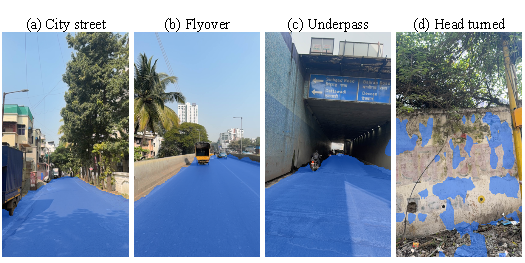
\includegraphics[width=\linewidth]{helmet_frames.pdf}
\caption{Road masks (blue) predicted on helmet-camera frames from the new rides: (a)--(c) correct masks on a city street, a flyover and an underpass entry; (d) a failure when the rider's head is turned towards a wall.}
\label{fig:helmet}
\end{figure}

\begin{table}[t]
\centering
\caption{Road-segmentation accuracy on BDD100K seg val (299 images) using the IDD-trained checkpoint.}
\label{tab:seg}
\setlength{\tabcolsep}{4pt}
\begin{tabular}{@{}p{0.55\linewidth}p{0.38\linewidth}@{}}
\toprule
\textbf{Metric} & \textbf{Value}\\
\midrule
Road IoU (micro)            & 0.856\\
Precision / recall (micro)  & 0.904 / 0.942\\
F1 (micro)                  & 0.922\\
Pixel accuracy              & 0.959\\
Per-image IoU               & 0.830 $\pm$ 0.177\\
\bottomrule
\end{tabular}
\end{table}

\subsection{System footprint and measured latency}
\label{sec:footprint}
Table~\ref{tab:footprint} lists the measured footprint and latency. On a laptop CPU, CV inference dominates the end-to-end detection-to-instruction latency (76.9\,ms mean); navigation-server round-trips are two orders of magnitude smaller. Because perception runs on the companion phone, never on the helmet microcontroller unit (MCU), we also measured the model on the target device: the checkpoint was exported to the Open Neural Network Exchange (ONNX) format, which gives per-pixel predictions identical to PyTorch, and run on an iPhone 17 Pro Max in Safari with ONNX Runtime Web. Inference takes 15.7\,ms on the phone GPU, whose output matched the CPU result on every pixel, and 35.9--54.1\,ms on the CPU. Against a 15\,m manoeuvre-approach window at 15\,m/s ($\approx$1\,s), even the slowest configuration leaves about 17$\times$ headroom. Power was measured by battery drain over two 30\,min runs at fixed brightness: 0\,\% with the page idle and 17\,\% with the model running continuously on the GPU (90{,}360 inferences). Scaled to 5 frames per second, about five frames inside the manoeuvre window, this is 3.0--3.6\,\% of battery per hour, the range reflecting the 1\,\% resolution of the battery indicator.

\begin{table}[t]
\centering
\caption{Measured footprint, latency and power: laptop CPU (PyTorch, \texttt{FastAPI} server) and the companion smartphone (iPhone 17 Pro Max, ONNX Runtime Web in Safari).}
\label{tab:footprint}
\setlength{\tabcolsep}{4pt}
\begin{tabular}{@{}p{0.53\linewidth}p{0.4\linewidth}@{}}
\toprule
\textbf{Metric} & \textbf{Value}\\
\midrule
Segmentation params / checkpoint     & 3{,}222{,}558 / 38.99 MB\\
Laptop CV inference ($N{=}30$) & 75.2 / 85.4 ms (mean/p95)\\
End-to-end detect$\rightarrow$instruction & 76.9 / 86.8 ms (mean/p95)\\
Laptop peak RAM (model / total) & 103 / 393 MB\\
\midrule
Phone, CPU 1 thread & 54.1 / 60.3 ms (mean/p95)\\
Phone, CPU 4 threads & 35.9 / 46.7 ms (mean/p95)\\
Phone, GPU (WebGPU) & 15.7 / 16.8 ms (mean/p95)\\
Phone runtime memory & 42.9 / 44.0 MB (1 / 4 thr.)\\
Phone battery, 30 min idle & 0\,\% (86\,\%$\rightarrow$86\,\%)\\
Phone battery, 30 min GPU (50.2 inf./s) & 17\,\% (86\,\%$\rightarrow$69\,\%)\\
Est.\ battery at 5 frames/s & 3.0--3.6\,\% per hour\\
\bottomrule
\end{tabular}
\end{table}

% ==============================================================
\section{Discussion and Limitations}
\label{sec:disc}
% ==============================================================

The evaluation has four limitations, each of which defines planned work. First, the seven rides were recorded by one rider in one city, and the six new rides are short; they show that the effect generalises across routes and road types, but not yet across riders, cities or weather. Second, GNSS outages are synthesised, because the recorded underpass and flyover did not interrupt the phone's GNSS fix; absolute errors are therefore indicative, while the paired contrasts, which share identical conditions, carry the main result. Third, the helmet-camera frames are unlabelled and sampled every 10\,s, so they show qualitative robustness to viewpoint and lighting rather than a pixel-level score, and the ablation's junction events remain geometric rather than visual. Fourth, the phone latency, memory and power measurements were taken only for the segmentation model running in a browser, which is slower than a native app, so the results are a conservative estimate. Power was estimated from battery drain measured in 1\,\% steps rather than with a power meter. Power consumption on the helmet side was not measured. Within these limits, GNSS ground truth is itself uncertain (median 14.2\,m), speed is held constant through each blackout in the absence of a wheel-speed sensor, and crash detection is a threshold-based SOS trigger rather than a certified diagnostic.

% ==============================================================
\section{Conclusion and Future Work}
\label{sec:conc}
% ==============================================================

This paper presented a hybrid offline navigation framework in which dead reckoning and vision-based road-feature detection preserve route continuity when GNSS is unavailable, by maintaining a route pointer over cached map data. On an instrumented road ride, the complete system reduced peak position error by 19.7\,\% compared with unaided dead reckoning across 47 paired GNSS blackouts ($p{=}0.002$). This improvement held across 23 of 24 threshold settings and was also confirmed on six additional rides: pooled over all seven rides, peak position error decreased by 20.6\,\% across 85 windows ($p{<}0.001$). However, junction correction without route context showed no measurable benefit. The segmentation backbone reached 0.856 road IoU on unseen BDD100K imagery and found the road ahead in 54 of 56 helmet-camera frames, and inference took 15.7\,ms on the companion smartphone. The main contribution is architectural: treating offline two-wheeler navigation as feature-aware route-pointer progression with confidence-managed fallback.

Future work will (i) record longer rides by several riders, including long tunnels that cause genuine GNSS outages; (ii) record continuous, pixel-labelled helmet-camera video so that junction events are produced by the vision pipeline and the effects of viewpoint, vibration, illumination and occlusion can be quantified; (iii) measure smartphone and helmet power with an inline meter; (iv) add a wheel-speed input to remove the constant-velocity assumption; and (v) resolve the remaining navigation-suite failures.

% ==============================================================
\section*{Acknowledgment}
% ==============================================================

The authors thank the School of Computer Engineering and Technology, MIT World Peace University, Pune, for supporting this work. An AI tool was used only for language editing.

% ==============================================================
\bibliographystyle{IEEEtran}
\bibliography{refs}

\end{document}
